%% ****** Start of file aiptemplate.tex ****** %
%%
%%   This file is part of the files in the distribution of AIP substyles for REVTeX4.
%%   Version 4.1 of 9 October 2009.
%%
%
% This is a template for producing documents for use with 
% the REVTEX 4.1 document class and the AIP substyles.
% 
% Copy this file to another name and then work on that file.
% That way, you always have this original template file to use.

%\documentclass[aip,graphicx]{revtex4-1}
%\documentclass[aip,reprint]{revtex4-1}

%\usepackage{graphicx}

%\draft % marks overfull lines with a black rule on the right
%\documentclass[pre,aps,floatfix,authordate1-4,twocolumn]{revtex4-1}
%\documentclass[pre,aps,floatfix,authordate1-4]{revtex4-1}

\documentclass[aps,prl,superscriptaddress,twocolumn]{revtex4}



%\documentclass[aps,prl,preprint,groupedaddress]{revtex4}

\usepackage{rotating} 
\usepackage{times}
\usepackage{graphicx}
\usepackage{setspace}
\usepackage{amsmath}
\usepackage{epstopdf}
\usepackage[obeyFinal]{easy-todo}
\begin{document}

% Use the \preprint command to place your local institutional report number 
% on the title page in preprint mode.
% Multiple \preprint commands are allowed.
%\preprint{}

\title{Quantitative quality of lipid-cholesterol interactions in atomistic resolution molecular dynamics simulations} %Title of paper

% repeat the \author .. \affiliation  etc. as needed
% \email, \thanks, \homepage, \altaffiliation all apply to the current author.
% Explanatory text should go in the []'s, 
% actual e-mail address or url should go in the {}'s for \email and \homepage.
% Please use the appropriate macro for the type of information

% \affiliation command applies to all authors since the last \affiliation command. 
% The \affiliation command should follow the other information.

\author{Peter Heftberger}
%\email[]{samuli.ollila@aalto.fi}
%\homepage[]{Your web page}
%\thanks{}
%\altaffiliation{}
\affiliation{University of Graz}

\author{O. H. Samuli Ollila}
\email[]{samuli.ollila@aalto.fi}
%\homepage[]{Your web page}
%\thanks{}
%\altaffiliation{}
\affiliation{Aalto University}

\author{Georg Pabst}
\affiliation{University of Graz}

% Collaboration name, if desired (requires use of superscriptaddress option in \documentclass). 
% \noaffiliation is required (may also be used with the \author command).
%\collaboration{}
%\noaffiliation

\date{\today}

\begin{abstract}
% insert abstract here
The quantitative quality of lipid-cholesterol interactions in atomistic resolution models will be determined against 
NMR and scattering data.
\end{abstract}

%\pacs{}% insert suggested PACS numbers in braces on next line

\maketitle %\maketitle must follow title, authors, abstract and \pacs

% Body of paper goes here. Use proper sectioning commands. 
% References should be done using the \cite, \ref, and \label commands


%\label{}
\section{Introduction}
The quantitative quality of lipid-cholesterol interactions in atomistic resolution models will be determined against 
NMR and scattering data.

\section{Methods}

\subsection{X-ray scattering experiments}


This folder contains SAXS data on POPC multilamellar vesicles (MLVs) at various cholesterol concentrations. Data have been obtained at the EMBL BioSAXS beamline (Hamburg) using 20 keV photons, T = 27°C. Data were analyzed in terms of the SDP-GAP model described in Heftberger et al., J. Appl. Cryst. 2013 and Heftberger et al. Biophys. J. 2015. Data from MLVs are a convolute of structure factor (the crystalline lattice) and form factor. By fitting the scattered intensity data we obtain both contributions. Here we posted only form factors (ASCII format). For information on the quality of the fit we also give plots of the fitted intensity data. The electron density profile has been modelled in terms of the SDP model (see papers by Kucerka and coworkers), that is volume distribution functions are modelled by individual Gaussians or error functions. Cholesterol is also accounted for by two Gaussians. This model has been proposed by Jianjun Pan (USF, Tampa, FL), but is to the best of our knowledge not published (see also PhD Thesis by Peter Heftberger). Additional figures show the volume distribution functions and the resulting electron density profiles.

Authors to consult and potentially include in publications using this data: Peter Heftberger (peter.heftberger@gmx.at), Georg Pabst (georg.pabst@uni-graz.at)
\subsection{Molecular dynamics simulations}
\begin{table*}[]
\centering
\caption{Simulated lipid bilayers containing cholesterol. The simulation file data sets marked with $^*$ include also part of the trajectory.
$^a$ The number of lipid molecules
$^b$ The number of cholesterol molecules
$^c$ Cholesterol concentration (mol\%)
$^d$ The number of water molecules
$^e$ Simulation temperature
$^f$ The total simulation time
$^g$ Time frames used in the analysis
$^h$ Reference link for the downloadable simulation files
$^i$ Reference for the full simulation details
}\label{systemsCHOL}
\begin{tabular}{c c c c c c c c c c c}
%\hline
Force field & lipid   & $^a$N$_{\rm l}$ & $^b$N$_{\rm chol}$ &$^c$C$_{\rm CHOL}$  &  $^d$N$_{\rm w}$ & $^e$T (K)  & $^f$t$_{{\rm sim}}$(ns)  & $^g$t$_{{\rm anal}}$ (ns)& $^h$Files  &  $^i$Details\\
\hline
Berger-POPC-07~\cite{ollila07a}&   POPC &128 & 0 &0\% & 7290  & 298  & 270 & 240 & [\citenum{bergerFILESpopc}]$^*$ & [\citenum{ferreira15}] \\
/H\"oltje-CHOL-13~\cite{holtje01,ferreira13}   &    & &  &   &   &  &  &  &  \\
                               &   POPC &120 & 8 & 6\% &7290   & 298  & 100 & 80 & [\citenum{bergerFILESpopc7chol}]$^*$ & [\citenum{ferreira13}] \\
                               &   POPC &110 & 18& 14\% & 8481  & 298  & 100 & 80 & [\citenum{bergerFILESpopc15chol}]$^*$ & [\citenum{ferreira13}]  \\
                               &   POPC &84 & 44 & 34\%  & 6794   & 298  & 100 & 80 & [\citenum{bergerFILESpopc34chol}]$^*$ & [\citenum{ferreira13}] \\
                               &   POPC &64 & 64 & 50\% & 10314  & 298  & 100 & 80 & [\citenum{bergerFILESpopc50chol}]$^*$ & [\citenum{ferreira13}] \\
                               &   POPC &50 & 78 & 61\% & 5782   & 298  & 100 & 80 & [\citenum{bergerFILESpopc60chol}]$^*$ & [\citenum{ferreira13}] \\
CHARMM36\cite{klauda10,lim12}   & POPC   & 128& 0& 0\% & 5120  & 303  & 150 & 100 & [\citenum{charmm36files}]$^*$  &  [\citenum{botan15}]  \\
%                                & POPC   & 512& 0& 0\% & 23943  & 298  & 170 & 100 & [\citenum{charmmPOPC512files}]$^*$  & SI  \\
%                                & POPC   & 460& 52& 10\% & 23569  & 298  & 170 & 100 & [\citenum{charmmPOPC512files}]$^*$  & SI  \\
%                                & POPC   & 436& 76& 15\% & 23331  & 298  & 170 & 100 & [\citenum{charmmPOPC512files}]$^*$  & SI  \\
                                & POPC   & 100 & 24 & 19\%  &  4960   & 303 & 200 & 100 & [\citenum{charmm36files20perCHOL}]$^*$ & [\citenum{botan15}] \\
%                                & POPC   & 410& 102& 20\% & 20972  & 298  & 170 & 100 & [\citenum{charmmPOPC512files}]$^*$  & SI  \\
%                                & POPC   & 384& 128& 25\% & 22327  & 298  & 170 & 100 & [\citenum{charmmPOPC512files}]$^*$  & SI  \\
%                                & POPC   & 332& 180& 35\% & 21340  & 298  & 170 & 100 & [\citenum{charmmPOPC512files}]$^*$  & SI  \\
%                                & POPC   & 256& 256& 50\% & 20334  & 298  & 170 & 100 & [\citenum{charmmPOPC512files}]$^*$  & SI  \\
                               & POPC   & 80 & 80 &50\%  &  4496    & 303 & 200 & 100 & [\citenum{charmm36files50perCHOL}]$^*$ & [\citenum{botan15}] \\
MacRog\cite{kulig15b}     & POPC   & 128 & 0 & 0\% & 6400  & 310 & 400 & 200 & [\citenum{macrogCHOLfiles}]$^*$ & [\citenum{botan15}] \\ 
                          & POPC   & 114  & 14 & 11\% & 6400  & 310  & 400 & 200 & [\citenum{macrogCHOLfiles}]$^*$ & [\citenum{botan15}]    \\
                          & POPC   & 72   & 56 &  44\% & 6400  & 310  & 400 & 200 & [\citenum{macrogCHOLfiles}]$^*$ & [\citenum{botan15}]    \\
                             & POPC   & 64  & 64 & 50\% & 6400  & 310  & 400 & 200 & [\citenum{macrogCHOLfiles}]$^*$ & [\citenum{botan15}]    \\
                             & POPC   & 56   & 72 & 56\% & 6400  & 310  & 400 & 200 & [\citenum{macrogCHOLfiles}]$^*$ & [\citenum{botan15}]    \\
\end{tabular}
\end{table*} 


\section{comparison of acyl chain order parameters between experiments and simulations}
Order parameters from simulations and experiments for acyl chains of 1-palmitoyl-2-oleoylphosphatidylcholine (POPC)
are shown in Fig. \ref{OrderParametersCHOL}.
 \begin{figure*}[]
  \centering
  \includegraphics[width=17.2cm]{../FIGS/OrderParametersCHOL.eps}

  \caption{\label{OrderParametersCHOL}
    Order parameters from simulations and experiments for acyl chains of  1-palmitoyl-2-oleoylphosphatidylcholine (POPC).}

  \todo{Why are the order parameters of CHARMM36 too large compared to simulations even without cholesterol? 
    Discussion in https://github.com/NMRLipids/NmrLipidsCholXray/issues/4}  

  \todo{Why there is decrease in order parameters towards beginning of acyl chain in MacRog model without cholesterol?}

  \todo{Do the results suggests that condensation effect is too strong in MacRog and Berger models?
  Discussion in https://github.com/NMRLipids/NmrLipidsCholXray/issues/5}
\end{figure*}

The order parameter changes as a function of cholesterol for each segment are shown in Fig.~\ref{OrderParametersCHOLchanges}
(currently only sn-1).

 \begin{figure}[]
  \centering
  \includegraphics[width=8cm]{../FIGS/OrderParametersCHANGEScholSN1.eps}

  \caption{\label{OrderParametersCHOLchanges}
    Order parameter changes from simulations and experiments for each segment in sn-1 chain of  1-palmitoyl-2-oleoylphosphatidylcholine (POPC) as a function of cholesterol concentration.}

\end{figure}

\section{Comparison of form factors between experiments and simulations}
The form factors calculated from different simulations with different cholesterol content are shown in 
Fig.~\ref{FormFactors}.

 \begin{figure}[]
  \centering
  \includegraphics[width=8cm]{../FIGS/FormFactors.eps}

  \caption{\label{FormFactors}
    Form factors from simulations and experiments.
  }

  \todo{Form factor calculation method should be double checked.}

  \todo{Experimental form factor amplitudes are not scaled to match with simulations, as done usually}

  \todo{Not all experimental and simulation data is here.}
    
\end{figure}



\section{Conclusions}

% Tables may be be put in the text as floats.
% Here is an example of the general form of a table:
% Fill in the caption in the braces of the \caption{} command. Put the label
% that you will use with \ref{} command in the braces of the \label{} command.
% Insert the column specifiers (l, r, c, d, etc.) in the empty braces of the
% \begin{tabular}{} command.
%
% \begin{table}
% \caption{\label{} }
% \begin{tabular}{}
% \end{tabular}
% \end{table}

% If you have acknowledgments, this puts in the proper section head.
\begin{acknowledgments}
% Put your acknowledgments here.
\end{acknowledgments}
\newpage
\appendix
\begin{center}
{\bf SUPPLEMENTARY INFORMATION}
\end{center}
\section{CHARMM36 results from different simulation packages}
The results from CHARMM36 model for lipid bilayers from different 
simulation packages have been reported to give different results in
the literature \cite{piggot12,lee16}. The results are mainly
dependent on different Lennart-Jones cut--off settings, but
all the details are not quite understood. In this work we use
the results from Gromacs 5 with settings suggested to be optimal
by Gromacs webpage. We also compared the results from Gromacs 5 with
these settings to the results simulated with NAMD, OpenMM and literature
values. The comparison is shown in Fig. \ref{programsCOMP}
 \begin{figure}[]
  \centering
  \includegraphics[width=8cm]{../FIGS/OrderParametersPROGRAMS.eps}

  \caption{\label{programsCOMP}
    Results for CHARMM36 model \cite{klauda10} from different simulation packages.
    Discussion going on at {\it https://github.com/NMRLipids/NmrLipidsCholXray/issues/4}.
  }
\end{figure}

% Create the reference section using BibTe
\bibliography{refs.bib}

%\newpage
%\section{APPENDIX: The NMR results reported by Tiago Ferreira}

\listoftodos

\end{document}
%
% ****** End of file aiptemplate.tex ******
